\section{zy}

%---------------------------------------------------------
%Changing visivility of the text
\section{Prostate Cancer Example}

    \begin{frame}{Prostate Cancer Example}
        \begin{itemize}
            \item 8 predictors: log(cancer volume), log(prostate weight), age, the logarithm of the amount of benign prostatic hyperplasia, seminal vesicle invasion, log(capsular penetration), Gleason score and percentage Gleason score 4 or 5.
            \item The response is the logarithm of prostate-specific antigen.
        \end{itemize}
        
    \end{frame}

    \begin{frame}{OLS, Ridge Regression, LASSO and Elastic Net}
        \begin{itemize}
            \item OLS, ridge regression, the lasso, the naive elastic net and the elastic net were applied.
            \item Training set: 67 observations; Test set: 30 observations.
            \item Model fitting and tuning parameter selection by tenfold CV were carried out on the training data.
        \end{itemize}
    \end{frame}

    \begin{frame}{Comparison}
        \begin{figure}
            \centering
            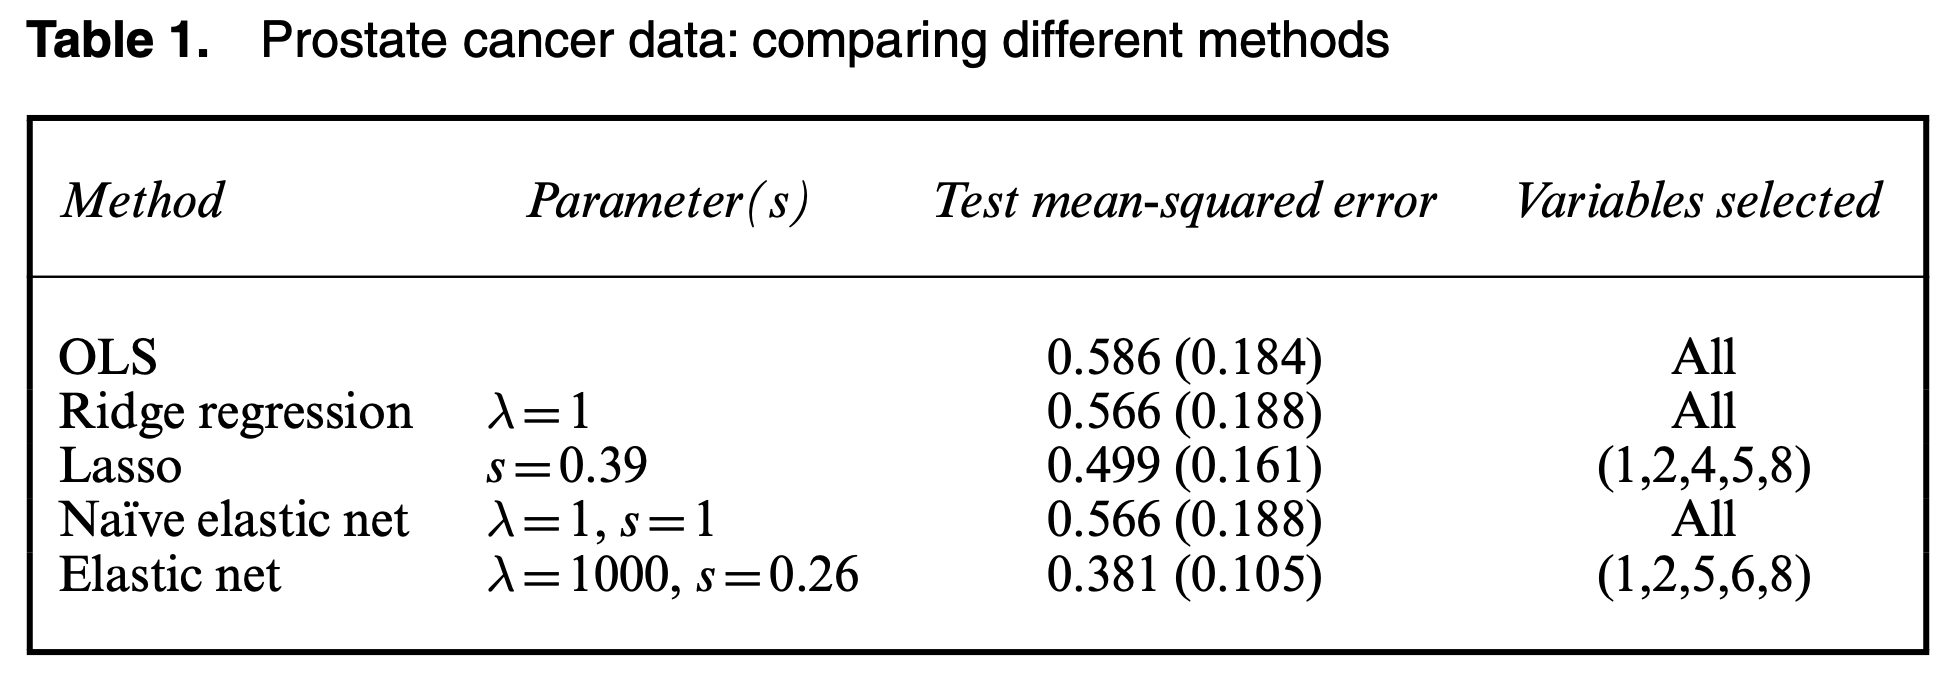
\includegraphics[width=0.6\textwidth]{img/sim/Table 1.png}
            % \caption{Caption}
            \label{fig:enter-label}
        \end{figure}
        \begin{itemize}
            \item Elastic net is the winner in terms of both prediction accuracy and sparsity.
            \item OLS is the worst.
            \item Naive elastic net is identical to ridge regression.
            \item The prediction error: elastic net is about 24\% lower than lasso.
            \item Elastic net is UST(Univariate Soft thresholding), because $\lambda$ selected is very big.
        \end{itemize}
    \end{frame}
\section{Simulation Study}
    
    \begin{frame}{Simulation}
    \begin{itemize}
        \item The simulated data comes from the true model: $y=x\beta+\sigma\epsilon,\epsilon\sim N(0,1).$ 
        \item Each simulated dataset is divided into training set/ validation set/ test set to serve. Models were fitted on the training set only, and the validation data were used to select the tuning parameters.
        \item The test error (the mean-squared error) was computed on the test set.

    \end{itemize}
    \end{frame}

    \begin{frame}{Simulation Example 1 and 2}
    \begin{itemize}
        \item Simulation example 1: 50 data sets were simulated consisting of 20/20/200 observations and 8 predictors:

$$
\beta=(3,1.5,0,0,2,0,0,0), \sigma=3
$$
$$
 \text{and cov}( x_i, x_j) = ( 0.5) ^{|i- j|} \text{ for all } i,j=1,...,8.
$$
        \item Simulation example 2: Same as example 1, except $\beta_j=0.85$ for all $j.$
    \end{itemize}
    \end{frame}

    \begin{frame}{Simulation Example 3}
        \begin{itemize}
            \item Simulation example 3: 50 data sets were simulated consisting of 100/100/400 observations and 40 predictors:
            
 $$\beta= ( \underbrace{0, ...,0}_{10} ,\underbrace{2, ..., 2}_{10}, \underbrace{0, ...,0}_{10} ,\underbrace{2, ..., 2}_{10}) $$ 
 $$ \text{and } \sigma= 15,  \text{cor}( x_i, x_j) = 0.5 \text{ for all }i,j=1,...,40.$$
        \end{itemize}
    \end{frame}


    \begin{frame}{Simulation Example 4}
        \begin{itemize}
            \item Simulation example 4: 50 data sets were simulated consisting of 50/50/400 observations and 40 predictors:

$$\beta= ( \underbrace{3, ..., 3}_{15}, \underbrace{0, ..., 0}_{25}) , \text{and }\sigma=15.$$

$$\mathbf{x}_{i}=Z_1+\epsilon_i^X,\quad Z_1\sim N(0,1),\quad i=1,...,5.$$

$$\mathbf{x}_{i}=Z_2+\epsilon_i^X,\quad Z_2\sim N(0,1),\quad i=6,...,10.$$

$$\mathbf{x}_{i}=Z_2+\epsilon_i^X,\quad Z_2\sim N(0,1),\quad i=11,...,15.$$
 $$\mathbf{x}_{i}\overset{\mathrm{i.i.d.}}{\operatorname*{\sim}}N(0,1),\quad i=16,...,40$$
 $$\epsilon_i^x\stackrel{\mathrm{i.i.d.}}{\sim}N(0,0.01),\quad i=1,...,15$$
            
        \end{itemize}
    \end{frame}

    \begin{frame}{Simulated Examples - Median MSE}
        \begin{figure}
            \centering
            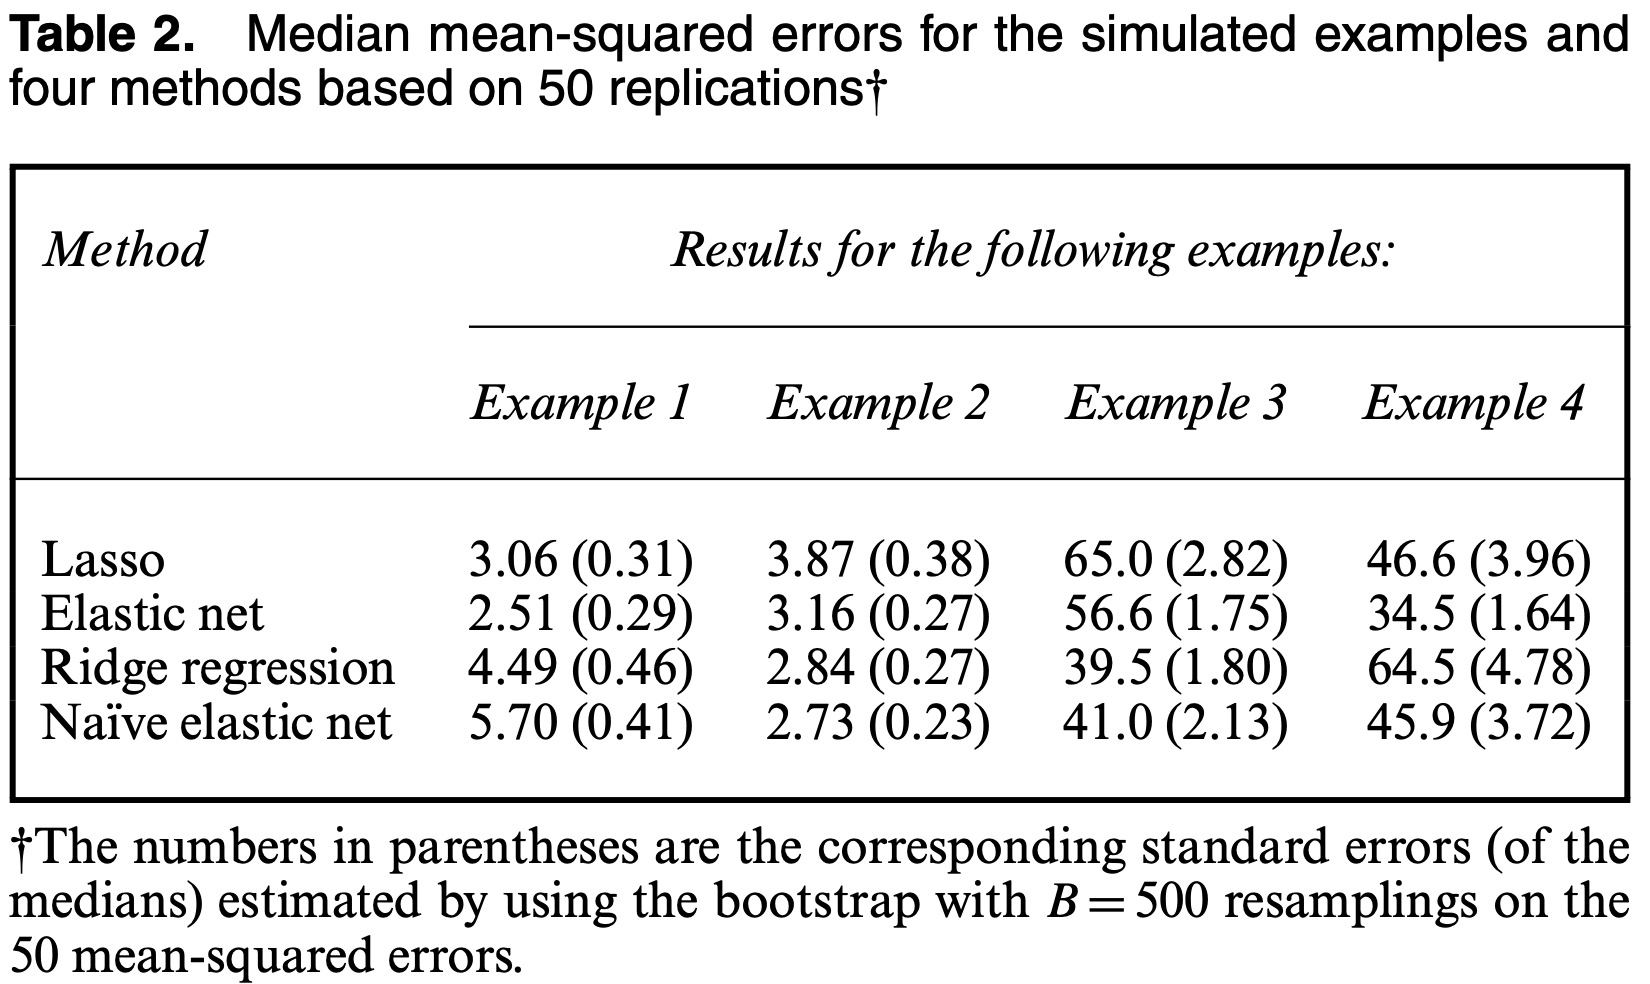
\includegraphics[width=0.6\textwidth]{img/sim/Table 2.png}
            % \caption{Caption}
            \label{fig:enter-label}
        \end{figure}
        \begin{itemize}
            \item Elastic Net is more accurate than the LASSO in all four examples, even when the LASSO is significantly more accurate than Ridge regression.
            \item The Naive Elastic Net performs very poorly with the highest mean-squared error in Example 1. In Example 2 and 3 it behaves very similar to Ridge regression, and in Example 4 it behaves similar to the LASSO.
        \end{itemize}
    \end{frame}

    \begin{frame}{Simulated Examples - Median MSE}
        \begin{figure}
            \centering
            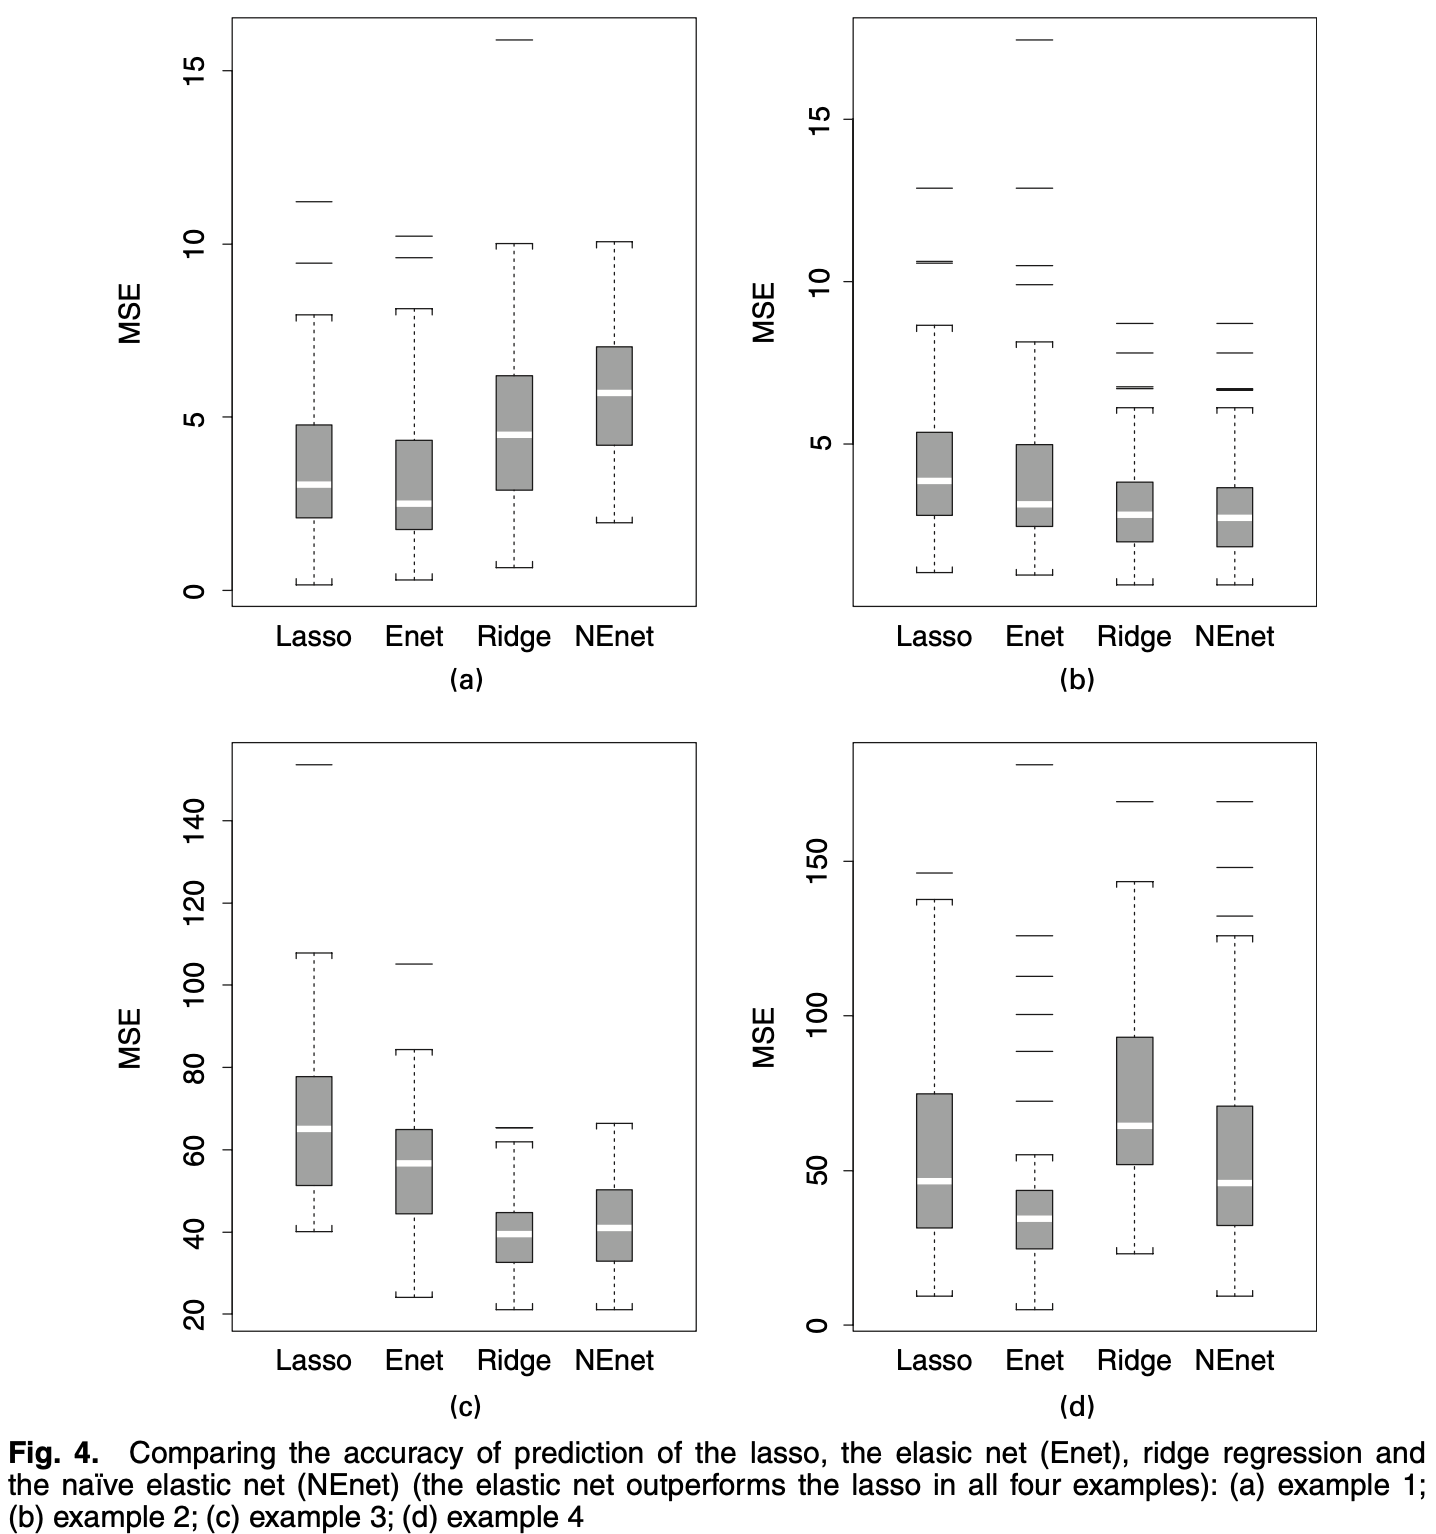
\includegraphics[width=0.45\textwidth]{img/sim/Fig 4.png}
            % \caption{Caption}
            \label{fig:enter-label}
        \end{figure}
        \begin{itemize}
            \item Using the box-plot, the overall prediction performance of the LASSO, ridge, elastic net, and naive elastic net is compared for 4 example.
        \end{itemize}
    \end{frame}

    \begin{frame}{Simulated Examples - Variable Selection}
        \begin{figure}
            \centering
            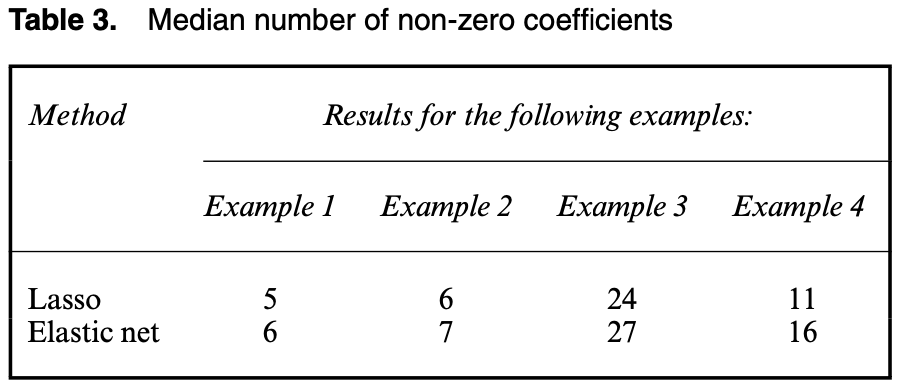
\includegraphics[width=0.6\textwidth]{img/sim/Table 3.png}
            % \caption{Caption}
            \label{fig:enter-label}
        \end{figure}
        \begin{itemize}
            \item Elastic Net selects more predictors than the LASSO due to the grouping effect. 
            \item Elastic Net behaves like the ideal model in Example 4, where grouped selection is needed.
            \item Therefore, the Elastic Net has the additional ability to perform grouped variable selection, which makes it a better variable selection method than the LASSO.

        \end{itemize}
    \end{frame}
    \begin{frame}{Conclusion}
    \begin{itemize}
        \item The LASSO can select at most $n$ predictors in the $p>n$ case and cannot perform grouped selection. Furthermore, the ridge regression usually has a better prediction performance than the LASSO when there are high correlations between predictors in the $n>p$ case.
        \item The Elastic Net can produce a sparse model with good prediction accuracy, while
 selecting group(s) of strongly correlated predictors. It can also potentially select all $p$
 predictors in all situations.
        % \item A new algorithm called LARS-EN can be used for computing elastic net regularization
 paths efficiently, similar to the LARS algorithm for LASSO.
        \item The Elastic Net has two tuning parameters as opposed to one tuning parameter like the LASSO, which can be selected using a training and validation set.
        \item Simulation results indicate that the Elastic Net dominates the LASSO, especially
 under collinearity.
    \end{itemize}
        
    \end{frame}

%---------------------------------------------------------
